\chapter{Introduzione alle proteine}
\section{Composizione e struttura delle proteine}
Le proteine sono macromolecole biologiche di natura polimerica costituite da catene di amminoacidi legati tra loro da un legame peptidico. La lunghezza della catena e la sequenza di amminoacidi, i principali sono venti, sono codificate geneticamente. È possibile individuare una catena principale, che consiste nella spina dorsale della molecola, alla quale risultano collegate le catene laterali, ossia le parti dei residui che rimangono libere, come mostrato in Figura~\ref{fig:backbone}. \cite{protein_physics}
\begin{figure}[h]
\centering
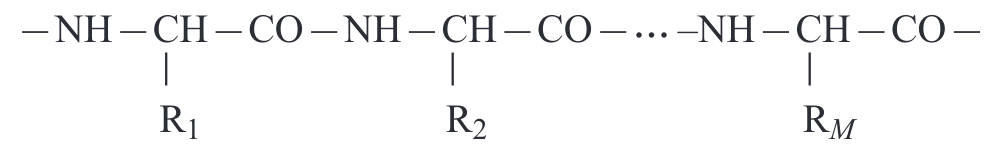
\includegraphics[width=9cm]{/home/michele_puppin/Scrivania/stesura_tesi/immagini/backbone.png}
\caption{Raffigurazione della catena principale. \cite{protein_physics}}
\label{fig:backbone}
\end{figure}

\noindent Le proteine svolgono molteplici funzioni a livello intra e extra cellulare. La maggior parte delle proteine ha funzioni di catalisi enzimatica delle reazioni chimiche svolgendo attività di regolazione nell'espressione genica, sintesi di molecole e ricezione e trasporto di informazioni. Sono inoltre ampiamente utilizzate come proteine di struttura o per il trasporto di altre molecole. 
Al fine di svolgere tale funzione è di cruciale importanza la struttura tridimensionale che le proteine assumono successivamente al loro assemblaggio. Queste infatti  hanno un'elevata specificità in relazione alle molecole con cui interagiscono e questo è spesso dovuto ad una interazione del tipo \textit{chiave-serratura} che richiede una rigida struttura spaziale. Qualora questa risultasse variata anche in minima parte, il funzionamento della proteina risulterebbe compromesso. \cite{protein_physics}

Alla base della catena proteica vi è l'unità peptidica rappresentata in Figura~\ref{fig:peptide_unit}. Questa presenta una configurazione planare a causa della natura del legame tra l'azoto e il carbonio che blocca la rotazione dell'angolo $ \omega $ rappresentato in Figura~\ref{fig:peptide_unit_2}. L'angolo $ \omega $ può unicamente vibrare a causa dell'agitazione termica ed è quindi fissato in modo tale da riprodurre la configurazione \textit{trans}, che risulta essere marcatamente più frequente, e \textit{cis}. 
L'angolo $ \chi $ rappresenta invece l'angolo di rotazione della catena laterale. Questo angolo, assieme alle vibrazioni della lunghezza dei legami, non contribuisce alla flessibilità della proteina e il contributo delle vibrazioni degli angoli è limitato: a conferire elevata flessibilità alla proteina sono quindi le rotazioni attorno agli angoli $ \psi $, $ \phi $. \cite{protein_physics}
\begin{figure}[h]
	\centering
	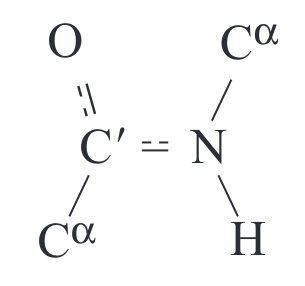
\includegraphics[width=2.5cm]{/home/michele_puppin/Scrivania/stesura_tesi/immagini/peptide_unit.png}
	\caption{Unità peptidica in configurazione \textit{trans}. \cite{protein_physics}}
	\label{fig:peptide_unit}
\end{figure}

\begin{figure}[h]
	\centering
	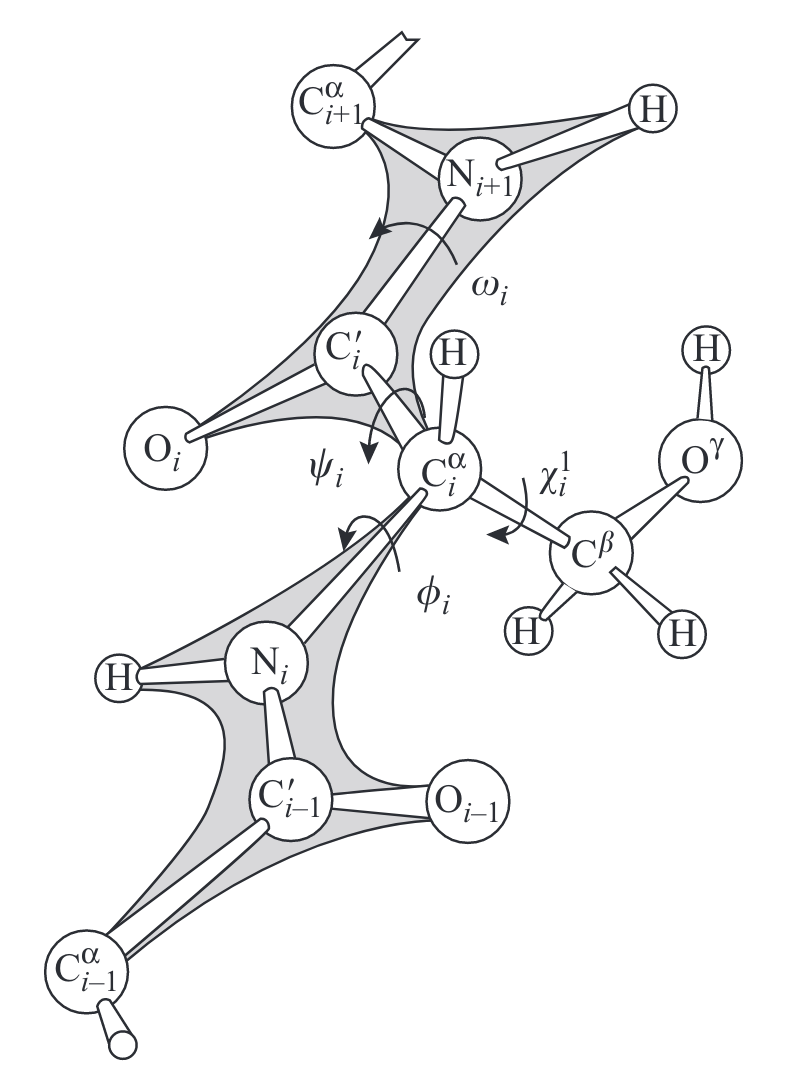
\includegraphics[width=6cm]{/home/michele_puppin/Scrivania/stesura_tesi/immagini/peptide_unit_2.png}
	\caption{Raffigurazione di una catena polipeptidica con il residuo i-esimo. \cite{protein_physics}}
	\label{fig:peptide_unit_2}
\end{figure}

La struttura proteica può essere studiata nel dettaglio tramite tecniche di cristallografia a raggi X e studi tramite risonanza magnetica nucleare della proteina in soluzione acquosa che permettono di ottenere le coordinate cartesiane dei singoli atomi. Questi approcci tuttavia sono possibili unicamente per lo studio di proteine solubili in acqua, ovvero le proteine globulari, in quanto possono essere facilmente isolate come molecole singole. Le proteine fibrose, così come le proteine di membrana, risultano invece insolubili in acqua ed è quindi difficile ricavarne la struttura. \cite{protein_physics}

La macrostruttura di una proteina può essere suddivisa in struttura primaria, secondaria, terziaria e quaternaria. La struttura primaria è data da una determinata sequenza di amminoacidi legati da legame peptidico. Sono invece generalmente legami non covalenti a mantenere la conformazione tridimensionale dando vita a strutture secondarie, terziarie e quaternarie. Le strutture secondarie sono ripiegamenti della catena polipeptidica nelle configurazioni $ \alpha $-\textit{elica} o $ \beta $-\textit{foglietto} raffigurate in Figura~\ref{fig:alfa_beta}. Le strutture  secondarie di una singola catena possono poi ripiegarsi in strutture globulari o fibrose che vanno quindi a costituire gran parte delle strutture terziarie esistenti. Infine l'associazione di più catene che interagiscono generalmente tramite legami deboli dà vita alle strutture quaternarie. Inoltre all'interno della singola catena si possono identificare due o più regioni compatte chiamate domini, generalmente contententi $ 100 $ - $ 200 $ residui, che svolgono funzioni specifiche. Ogni dominio ripiega in maniera autonoma.
Il ripiegamento della catena polipeptidica per formare strutture secondarie e terziarie avviene, \textit{in vitro}, spontaneamente e sempre nello stesso modo senza la necessità che intervengano processi cellulari specifici, che sono invece presenti \textit{in vivo}. Questo fatto indica chiaramente che la struttura della proteina deriva unicamente dalla specifica sequenza di amminoacidi che la compongono. \cite{protein_physics}
\begin{figure}[h]
	\centering
	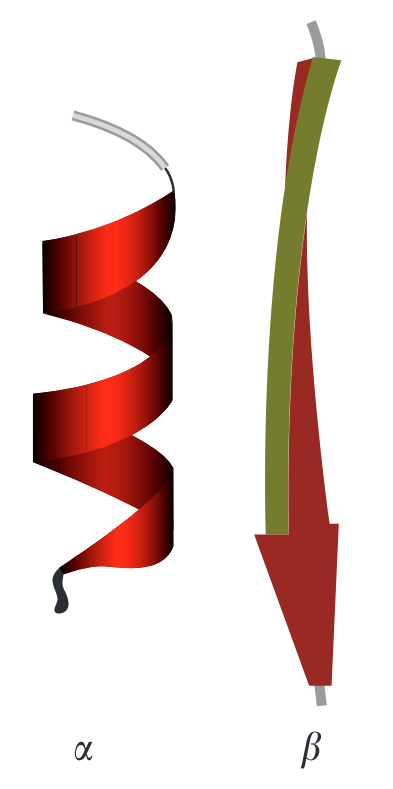
\includegraphics[width=3cm]{/home/michele_puppin/Scrivania/stesura_tesi/immagini/alfa_beta.png}
	\caption{Raffigurazione delle configurazioni $ \alpha $-\textit{elica} e $ \beta $-\textit{foglietto}. \cite{protein_physics}}
	\label{fig:alfa_beta}
\end{figure}

A determinare e mantenere le strutture secondarie e terziarie concorrono diversi tipi di interazione. Vi è la possibilità che si formi un ponte disolfuro tra due differenti residui di cisteina contenenti il gruppo $  - \mathrm{SH} $, ovvero un legame covalente del tipo $  - \, \mathrm{S} - \mathrm{S} - $. La maggior parte delle interazioni tuttavia è di natura non covalente.
Alcuni esempi sono  il legame ionico, dovuto essenzialmente all'interazione tra strutture con carica opposta come gruppi carbossilici carichi negativamente e gruppi amminici carichi positivamente, e le forze di Van der Waals, ovvero interazioni deboli ma fondamentali nello studio di agglomerati di grandi dimensioni. Queste sono dovute al fatto che a distanze superiori a $ 2 $ - $ 3 $ \AA{} gli atomi, invece di respingersi, si attraggono a causa delle vibrazioni coordinate degli elettroni in entrambi gli atomi.
Un'interazione molto più intensa delle forze di Van der Waals è invece il legame idrogeno; questo si instaura tra due residui quando un atomo di idrogeno legato ad un atomo elettronegativo si trova in prossimità di un altro atomo elettronegativo come nei casi $ \mathrm{O} - \mathrm{H} ::: \mathrm{O} $ e $ \mathrm{N}  - \mathrm{H} ::: \mathrm{N} $. In particolare nelle proteine si possono realizzare legami idrogeno del tipo $ \mathrm{N}  - \mathrm{H} ::: \mathrm{O} $ fra l'azoto del gruppo amminico e l'ossigeno del gruppo carbonilico, entrambi situati sulla catena principale, che stabilizzano le strutture secondarie.   
Infine un ruolo importante nella determinazione della forma globulare della proteina è svolto dall'effetto idrofobico per il quale la proteina tende ad esporre all'acqua i residui polari racchiudendo quindi in una tasca idrofobica quelli apolari. \cite{protein_physics}

\section{Entanglement topologico}
L'assemblaggio nei ribosomi della sequenza di amminoacidi a partire dalle informazioni contenute nel DNA, produce una catena lineare. Questa, subito dopo essere stata assemblata, va incontro ad un processo di ripiegamento per mezzo del quale assume la specifica forma tridimensionale, chiamata stato nativo, che risulta biologicamente funzionale. All'interno della cellula il processo viene favorito dall'azione di enzimi specifici che tuttavia hanno il solo scopo di evitare contatti indesiderati con altre molecole all'interno della cellula. Si è visto infatti che le proteine sono capaci di ripiegarsi spontaneamente anche \textit{in vitro}. \cite{protein_physics} Il fatto quindi che a partire da una determinata sequenza di amminoacidi si ottenga in modo del tutto spontaneo la medesima configurazione è un chiaro indizio del fatto che lo stato nativo rappresenta uno stato di minimo dell'energia.
 
Il processo di ripiegamento risulta estremamente complesso e difficile da studiare, sorge dunque naturale domandarsi come questo possa avvenire senza incorrere in errori anche per configurazioni molto complicate. Non è stato del tutto compreso, ad esempio, come tale processo dia vita a proteine che presentano nodi nella topologia della loro struttura, le quali pur presentando una configurazione intricata sono state rilevate in discreto numero fra le proteine del Protein Data Bank (3\%). \cite{Jackson2017HowTF}
Lo studio di alcuni meccanismi del processo di ripiegamento può essere svolto a partire dall'analisi della configurazione geometrica dello stato nativo. Si è visto, ad esempio, che  conoscendo quali coppie di residui risultano in contatto reciproco è possibile ricavare informazioni su quali siano i nuclei di ripiegamento della proteina. \cite{lunghezza}
Nel caso di proteine dall'elevata complessità, lo studio di proprietà locali non è tuttavia esauriente ed è utile analizzare aspetti più generali della geometria come ad esempio il grado di entanglement topologico di un determinato stato nativo. La proteina può infatti essere pensata come una curva che, deformandosi necessariamente in modo continuo, può essere analizzata con studi di natura topologica. L'entanglement topologico indica l'interconnessione fisica tra due molecole o tra due parti di una stessa molecola. 
Lo studio di questo aspetto può fornire informazioni utili; si è verificato infatti che la distanza media lungo la 
catena tra due residui che, entrando in contatto reciproco, danno vita ad un loop della catena proteica risulta fortemente correlata con il tempo di ripiegamento della proteina stessa. \cite{lunghezza}

È dunque interessante interrogarsi circa gli effetti che il grado di entanglement della struttura proteica ha a livello energetico e per farlo è necessario valutare matematicamente questa quantità. A tale scopo si utilizza l'entanglement gaussiano, ovvero una generalizzazione dell'integrale di Gauss utilizzato per calcolare il linking number. \cite{preprint}
Il linking number di due curve chiuse è un parametro che descrive quante volte una curva gira attorno all'altra. In generale se tale parametro è nullo risulta possibile separare le due curve senza spezzarle mentre se è non nullo questa operazione non risulta possibile. In Figura~\ref{fig:link} un esempio di curve con linking number nullo (sinistra) e pari a uno (destra).
\begin{figure}[h]
	\centering	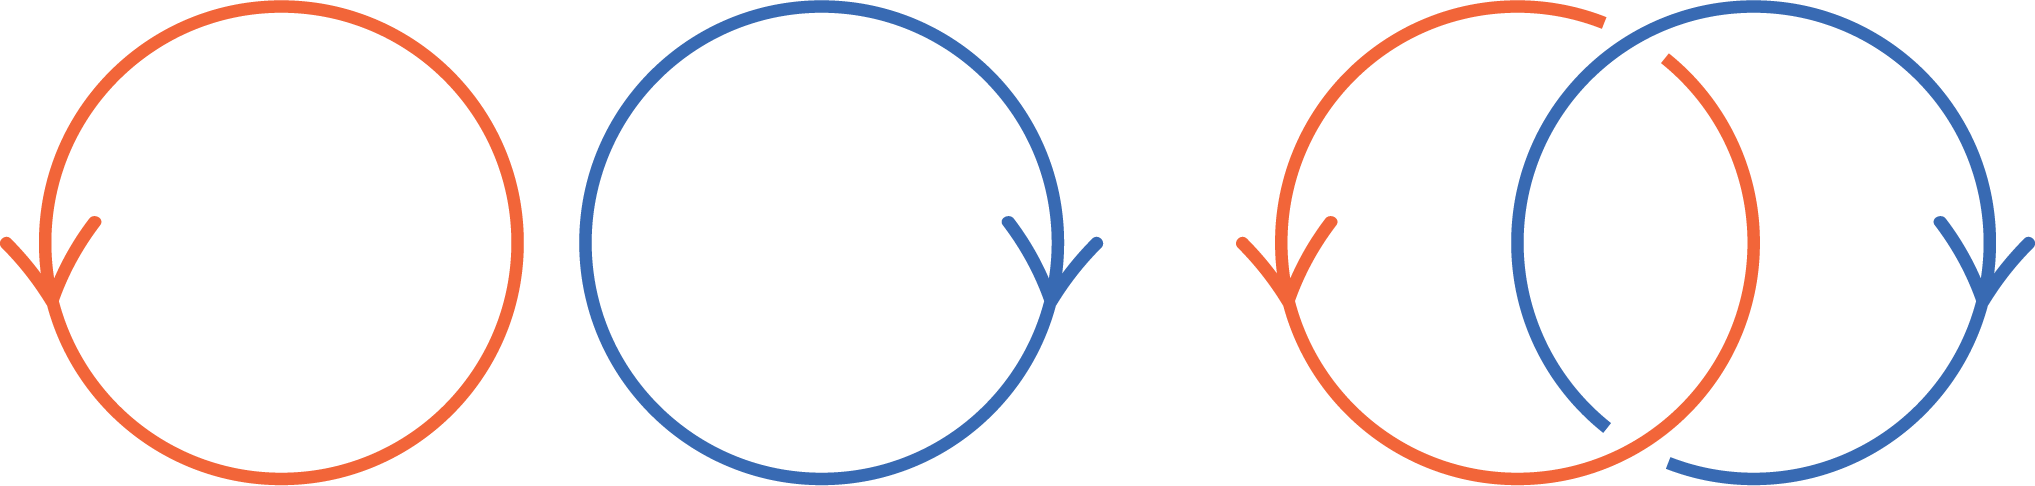
\includegraphics[width=8cm]{/home/michele_puppin/Scrivania/stesura_tesi/immagini/link.png}
	\caption{Due esempi di entanglement tra curve chiuse}
	\label{fig:link}
\end{figure}

Il linking number tra due curve chiuse $ \gamma_i = \{\mathbf{r}^{(i)}\} $ e $ \gamma_j = \{\mathbf{r}^{(j)}\} $ in $ \mathbb{R}^3 $ è un numero intero e un invariante topologico.
Il suo valore può essere calcolato tramite il doppio integrale di Gauss
\begin{equation}
G \equiv \frac{1}{4 \pi} \oint_{\gamma_i} \oint_{\gamma_j} \frac{\mathbf{r}^{(i)} - \mathbf{r}^{(j)}}{ \lvert \mathbf{r}^{(i)} - \mathbf{r}^{(j)} \rvert^3} 
\cdot (d\mathbf{r}^{(i)} \times d\mathbf{r}^{(j)}).
\label{eq:link}
\end{equation} 
Se si calcola il doppio integrale fra le due curve aperte invece si ottiene un numero reale $ G' $, chiamato entanglement gaussiano, che quantifica quindi proprio l'entanglement fra le due curve. \cite{Baiesi_2017}

Anche per le proteine è possibile calcolare l'entanglement gaussiano andando a prendere in considerazione due sottocatene, aperte o chiuse che siano. Un valore del modulo di $ G' $ maggiore, o al limite vicino, a uno indica una condizione di entanglement per le due sottocatene. All'interno delle strutture proteiche si possono venire a formare dei loop quando due residui in punti diversi della catena si trovano in contatto. Si è visto che conformazioni nelle quali due loop si intersecano, a sinistra in Figura~\ref{fig:link_prot}, o una parte della catena risulta avvolta da un loop, a destra in Figura~\ref{fig:link_prot}, risultano tutt'altro che rare, essendo presenti nel 30\% del data set di proteine a singolo dominio considerate in \cite{preprint}.
\begin{figure}[h]
	\centering
	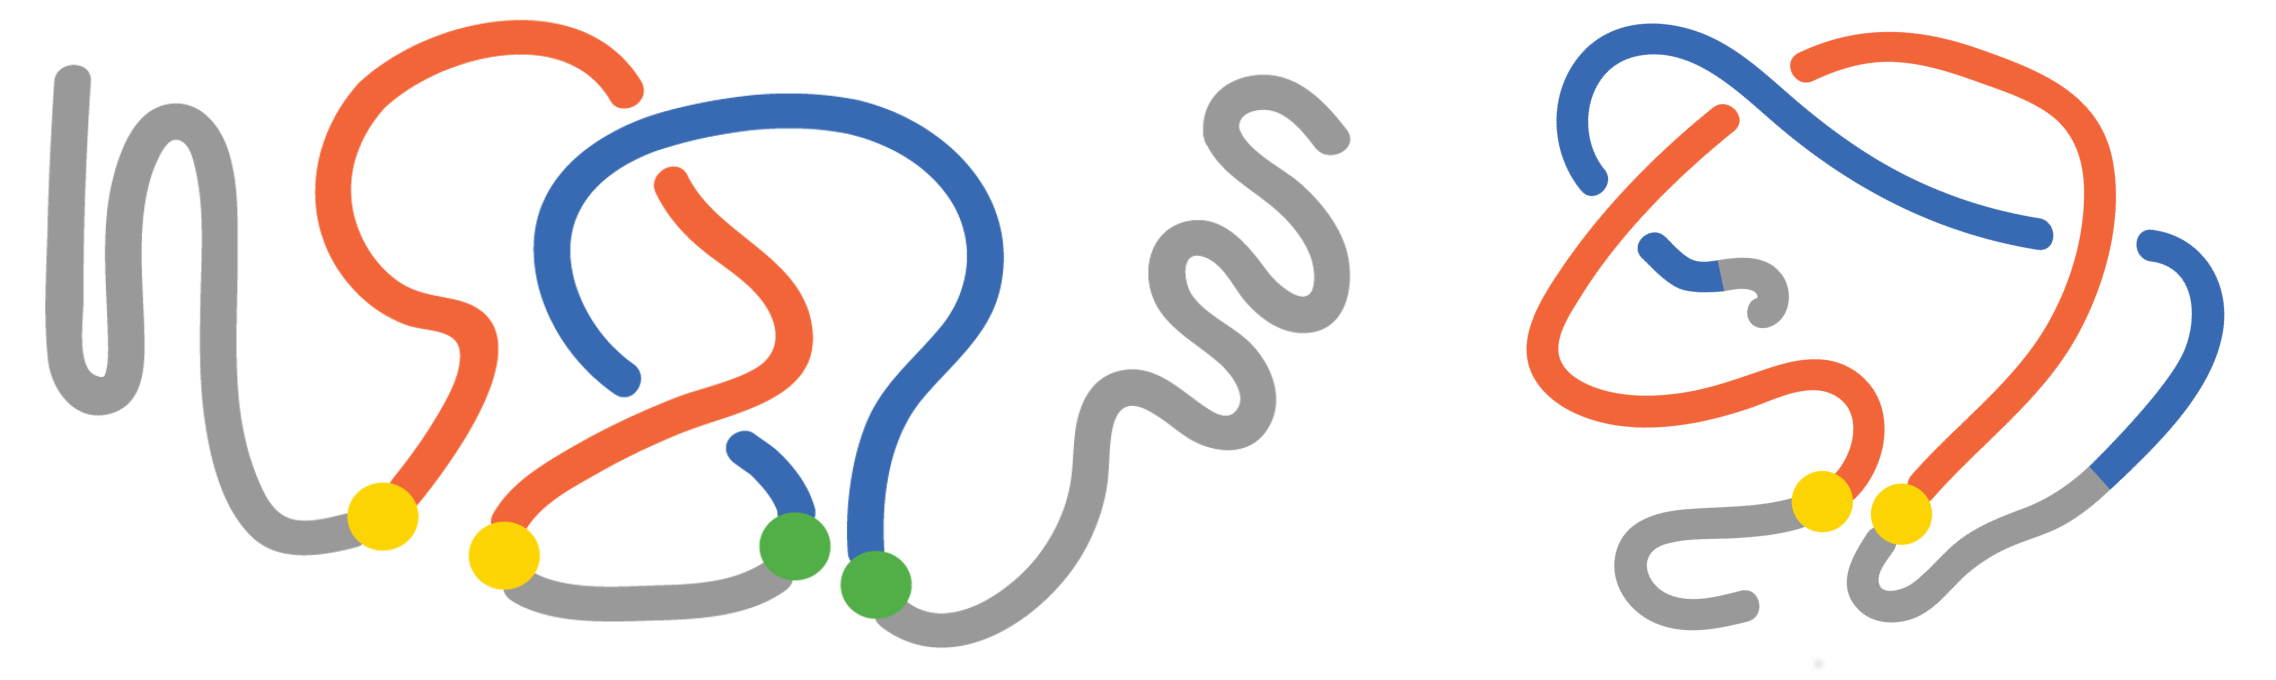
\includegraphics[width=9cm]{/home/michele_puppin/Scrivania/stesura_tesi/immagini/link_prot.png}
	\caption{Esempio di figure di entanglement proteico}
	\label{fig:link_prot}
\end{figure}

Per calcolare l'entanglement gaussiano a partire dalla proteina si prende in considerazione una catena peptidica e si traccia una linea spezzata che colleghi gli atomi di carbonio $ \mathrm{C}^{\alpha} $ consecutivi. È quindi possibile individuare le due sottocatene: la prima dal carbonio $ i_1 $ al carbonio $ i_2 $ corrisponderà alla curva $ \gamma_i $ mentre la seconda da $ j_1 $ a $ j_2 $ corrisponderà a $ \gamma_j $. Le due sottocatene devono essere tali che $ \gamma_i \cap \gamma_j = \emptyset $.
Risulta quindi possibile calcolare l'entanglement gaussiano come
\begin{equation}
G'_{ij} \equiv \frac{1}{4 \pi} \sum_{i=i_1}^{i_2-1} \sum_{j=j_1}^{j_2-1} \frac{\mathbf{R}_i - \mathbf{R}_j}{ \lvert \mathbf{R}_i - \mathbf{R}_j \rvert^3} \cdot (d\mathbf{R}_i \times d\mathbf{R}_j).
\label{eq:link_disc}
\end{equation}
Nella formula (\ref{eq:link_disc}) una proteina con $ N $ residui è pensata come una catena discreta di monomeri $ \left( i=1,...,N \right) $ aventi la posizione $ \mathbf{r}_i $ del carbonio $ \mathrm{C}^{\alpha} $ e si sono dunque definiti
\begin{equation}
\mathbf{R}_i \equiv \frac{1}{2} \left( \mathbf{r}_{i+1} + \mathbf{r}_i \right)
\qquad d\mathbf{R}_i =  \left( \mathbf{r}_{i+1} - \mathbf{r}_i \right)
\label{eq:pos_med}
\end{equation}
i vettori utilizzati nella (\ref{eq:link_disc}). \cite{Baiesi_2017}

  